\documentclass{standalone}
\usepackage{tikz}
\usepackage{esvect}
\usetikzlibrary{backgrounds}
\usepackage{xcolor}
\definecolor{plotblue}{RGB}{100, 100, 255}
\definecolor{myred}{RGB}{143,42,41}
\definecolor{forestgreen}{RGB}{34,139,34}
\definecolor{highdive}{RGB}{10,169,194}

\begin{document}
	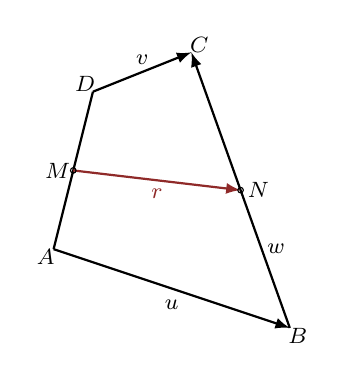
\begin{tikzpicture}[cross/.style={draw, cross out, minimum size=2*(#1-1pt), inner sep=0pt, outer sep=0pt}, x=10mm, y=10mm,
		>=latex,   %Voreinstellung für Pfeilspitzen
		font= \footnotesize, scale=0.5]
		%Vektoren
		\draw[->,thick] (0,0) -- (6,-2);
		\draw[->,thick] (6,-2) -- (3.5,5);
		\draw[<-,thick] (3.5,5) -- (1,4);
		\draw[thick] (0,0) -- (1,4);
		\draw[myred,->,thick] (0.5,2) -- (4.75,1.5);
		%Punkte
		\draw (0.5,2) circle (2pt);
		\draw (4.75,1.5) circle (2pt);
		%Beschriftung
		\node at (-0.2,-0.2) {$A$};
		\node at (6.2,-2.2) {$B$};
		\node at (3.7,5.2) {$C$};
		\node at (0.8,4.2) {$D$};
		\node at (0.1,2) {$M$};
		\node at (5.2,1.5) {$N$};
		\node[myred] at (2.625,1.4) {$\vv{r}$};
		\node at (3,-1.4) {$\vv{u}$};
		\node at (5.65,0) {$\vv{w}$};
		\node at (2.25,4.8) {$\vv{v}$};
	\end{tikzpicture}
\end{document}